\section{Qualitätsmessung der Kompression}
Um die Datenmenge der Feldlinien zu verringern werden verlustbehaftete Kompressionsverfahren angewendet. Trotz des Dateverlustes sollen die dekomprimierten Linien möglichst ihren Originalen ähneln. Es ist wichtig, dass die Form der Kurve. Grosse, seltene Abweichungen können das Aussehen beeinflussen.\\
[\baselineskip]
Im Verlauf der Arbeit wurden zwei unterschiedliche Metriken verwendet: Die Standardabweichung und eine angepasste PSNR-HVS-M. Für die ersten Messungen wurde die Standardabweichung gemessen. Es stellte sich heraus, dass die Metrik für den Anwendungsfall nicht ausreicht: Sichtbare Artefakte, wie hochfrequente Schwingungen um die Originallinie fallen nicht ins Gewicht. Wie die Standardabweichung berechnet wird, ist im Abschnitt \ref{testsetup:ablauf} beschrieben. Für weitere Messungen wurde eine angepasste PSNR-HVS-M Metrik verwendet. Es berücksichtigt nur Artefakte, die vom menschlichen Auge sichtbar sind.
%neu schreiben.
Zusammen mit Sonnenforschern wurden zwei Fehlermasse bestimmt: Der absolute maximale Fehler und die Standardabweichung von der komprimierten Linie zum Original. Die Standardabweichung ist für diesen Fall geeignet: Grosse, seltene Abweichungen werden stärker gewichtet, als kleine dafür häufige Abweichungen.\\
Der absolute maximale Fehler wird noch als Absicherung gemessen. In den meisten Fällen wird die Kompression mit der tieferen Standardabweichung auch den kleineren maximalen Fehler haben. Da aber die Messung über ein paar hunderttausend Punkte durchgeführt wird, ist das Gegenteil denkbar.\\
Subsample\\
[\baselineskip]
%meh
Eine Grenze für die Genauigkeit ist nicht festzulegen. Auch wenn eine Grenze gefunden wird, kann diese sich in der Zeit verändern. Im Fall der Feldlinien ist die Internetverbindung der Flaschenhals. Es kann sein, dass in Zukunft mehr Präzision bei mehr Platzbedarf verlangt wird. Deshalb werden die Verfahren, wenn möglich, mit unterschiedlichen Qualitätsstufen getestet und verglichen.

\subsection{Auswahl und Erhebung der Testdaten}\label{testsetup:auswahl_erhebung}
Die Testdaten sollen zu einem alle Randfälle abdecken, als auch durchschnittliche Fälle enthalten. Aus diesem Grund wurden insgesamt zehn Datensätze ausgewählt: Vier Datensätze mit hoher Sonnenaktivität, zwei mit wenig und vier zufällig. Für die vier Datensätzen mit hoher Aktivität wurde in den Jahren 2014 und 2013 nach den grössten Solare Flares gesucht. Für die Datensätze mit wenig Aktivität wurde das Gegenteil gemacht, nach Zeiträumen mit möglichst kleinen Solar Flares gesucht.\\
Die feldlinien werden aber nur alle sechs Stunden berechnet und Solar Flares sind sehr spontane Ereignisse. Auch eine grosse Flare kann während den sechs Stunden angefangen und wieder aufgehört haben. Für die grossen Solar Flares wurde deshalb beachtet, dass die Datensätze vor dem Ereignis verwendet wurden. Grosse Solar Flares entladen das Feld, vor dem Ereignis ist das Magnetfeld komplexer.\\
[\baselineskip]
Wie im Abschnitt \ref{konzept:ist-komprimierung} beschrieben, führt der IDL-Code schon eine Quantisierung und ein Subsampling durch. Für die Testdaten wurde das Subsampling und die Quantisierung entfernt. Für jede Dimension eines Punktes wird anstatt 16 Bit 32 Bit Genauigkeit verwendet. Die rohe Datenmenge ist dementsprechend Angewachsen auf etwa 10 MiByte pro Aufnahme.

\subsection{Berechnung der Standardabweichung}\label{testsetup:ablauf}
%Schlecht, nochmal
Float daten werden geladen. Daten kopiert und Kompression/Dekompression durchgeführt für alle Testdaten. Die kopierten Daten wissen aber noch, welches ihr Originalpunkt ist.
Zwei Mengen, Originalpunkte $O$, dekomprimierte Punkte $D$. Es gibt immer gleich viele oder mehr Originalpunkte wie dekomprimierte Punkte. Die Fehlerberechnung muss der allgemeine Fall und die Randbehandlung unterschieden werden.

\subsubsection{Allgemeiner Fall}
\begin{figure}[!htbp]
	\center
	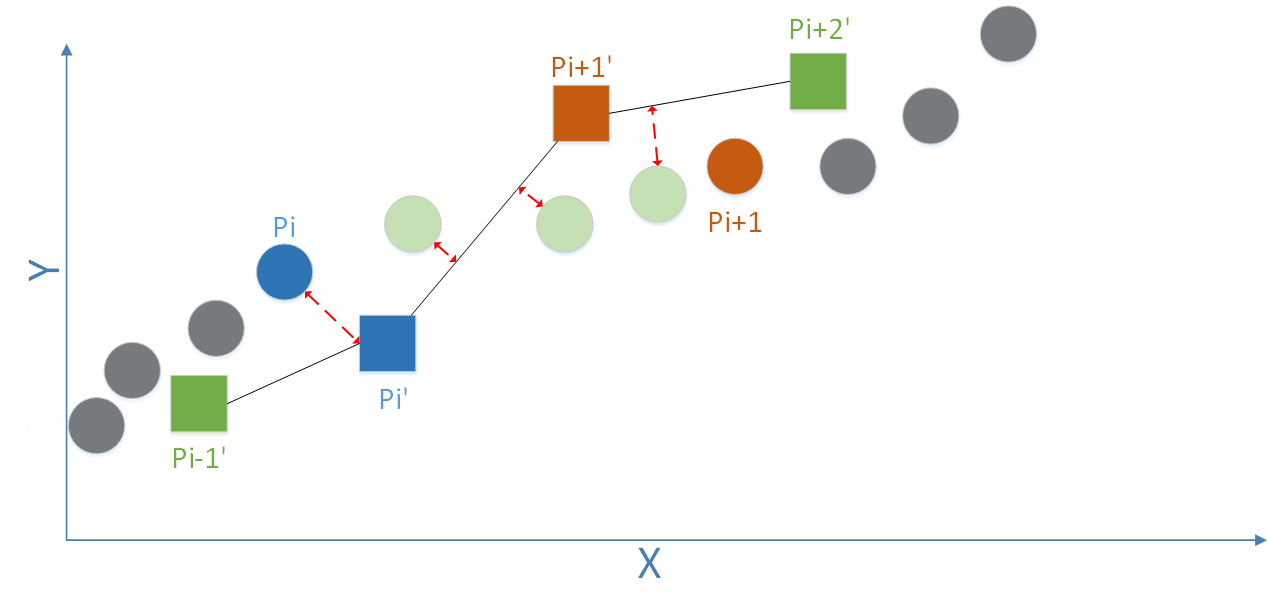
\includegraphics[width=0.8\textwidth,height=6cm,keepaspectratio]{./pictures/testsetup/errorcalc.png}
	\caption{Darstellung der Fehlerberechnung. Die Punkte sind die Originaldaten, die Quadrate sind die Punkte nach der Kompression.}
	\label{testsetup:ablauf:fehlerberechnung:diagramm}
\end{figure} 
Die Berechnung ist Dargestellt im Diagramm \ref{testsetup:ablauf:fehlerberechnung:diagramm}. Für jeden Punkt $p1'$ aus $D$, nehme $p1'$ und den folgenden Punkt und $P2'$. Ziehe eine Strecke $s$ durch $p1'$ und $p2'$. Suche von $p1'$ den Originalpunkt $P1$ aus $O$ und rechne den Abstand aus zur Strecke $s$. Führe das für alle folgenden Originalpunkte durch, bis $p2$ erreicht wurde. Der Abstand $s$ zu $p2$ wird nicht mehr berechnet.\\
[\baselineskip]
\textbf{Abstandsberechnung eines Punktes zu einer Strecke}\\
Gegeben: Stecke $s$ mit Eckpunkten $A$ und $B$ und Punkt $P$.\\
Gesucht: Kürzeste Distanz zwischen $s$ und $P$\\
[\baselineskip]
Zuerst wird überprüft, ob eine Senkrechte durch $P$ überhaupt auf der Strecke $s$ zu liegen kommt. Das ist der Fall, wenn die Strecke $AP$ auf die Strecke $s$ projizierbar ist:
\begin{center}
$ t = \frac{\vec{AB}*\vec{AP}}{\lvert \vec{AB}\rvert ^2}$\\
  $0 \leq t \leq 1$
\end{center}
Wenn das nicht möglich ist, wird der kürzere Distanz von $P$ zu einem der Eckpunkte genommen. Falls aber eine Senkrechte auf $s$ zu liegen kommt, muss jetzt die Länge der Senkrechte berechnet werden. Aus der vorhgehenden Berechnung könnte man den Fusspunkt auf $s$ berechnen und dadurch die Distanz, oder man kann die Distanz direkt über das Kreuzprodukt berechnen.
\begin{center}
  $distance = \frac{\lvert \vec{BA}\times \vec{BP}\rvert}{\lvert \vec{BP} \rvert}$
\end{center}

\subsubsection{Randbehandlung}
\begin{figure}[!htbp]
	\center
	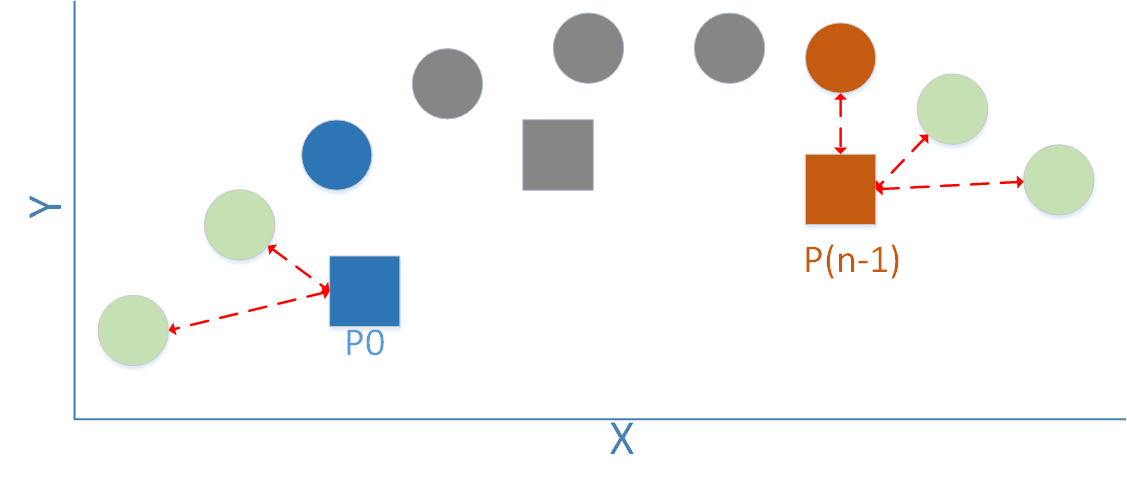
\includegraphics[width=0.8\textwidth,height=6cm,keepaspectratio]{./pictures/testsetup/randbehandlung.png}
	\caption{Darstellung der Fehlerberechnung. Die Punkte sind die Originaldaten, die Quadrate sind die Punkte nach der Kompression.}
	\label{testsetup:ablauf:randbehandlung:diagramm}
\end{figure}
Es ist möglich, dass die originalen Endpunkte durch eine Quantisierung verworfen wurden. Das bedeutet, wenn man den Fehler für den allgemeinen Fall berechnet, am Anfang und am Ende Originalpunkte existieren, für die nie eine Distanz berechnet wurde. Die Abbildung \ref{testsetup:ablauf:randbehandlung:diagramm} zeigt das Problem. Deshalb müssen die Abstände der Ränder von der Komprimierten- zur Original-Linie noch berechnet werden. Der Abstand vom ersten komprimierten Punkt (in der Abbildung P0) zu seinem Original wird schon im allgemeinen Fall berechnet.

\subsubsection{Berechnung der Standardabweichung}
\begin{center}
$\sigma(X) = \sqrt(variance(X))$\\
$variance(X) = \sum{(x_i - E(x_i))^2}$
\end{center}
Die Standardabweichung $\sigma$ einer Beobachtungsreihe $X$ $(x_1,x_2,x_3,\ldots, x_n-1)$ ergibt sich aus der Wurzel der Varianz von $X$. Die Varianz von $X$ kann errechnet werden, wenn man den Distanz jeder Beobachtung $x_i$ mit dem Erwartungswert $E(x_i)$ berechnet und quadriert. Die Beobachtung ist im diesen Fall ein Punkt der dekomprimierten Linie, während der Erwartungswert der Originalpunkt ist. Die Distanz wird mit dem besprochnen Verfahren \ref{testsetup:ablauf} berechnet. Die Summe der quadratischen Abstände ergibt die Varianz. Die Varianz wird über alle Testdaten berechnet, somit erhält man für einen Test genau eine Standardabweichung.

\subsection{Berechnung der angepassten PSNR-HVS-M}\label{testsetup:psnr}
grund dafür, ref auf resultate
Warum ist die Standardabweichung ungenügend: Mathematisch sinnvoll, aber die Daten werden schlussendlich von einem Menschen angeschaut. Gewisse Artefakte verschwinden, gewisse sind gut sichtbar. Ein sinnvolles mass für menschlichen Sehapparat zu finden ist ein aktives Vorschungsgebiet der Bildverarbeitung.

PSNR:

Verbesserung der PSNR-HVS

Awbwandlung

\subsubsection{Umsetzung}
Faktoren, Empirisch getestet mit algos. eher konservativ
maxvalue der psnr

\subsubsection{Wertebereich und Grenzen der PSNR}
Wann ist gut, wann knapp. Jetzt eher knapp